\documentclass[main.tex]{subfiles}
\begin{document}
实数域上的内积空间上的厄米算符、反厄米算符和幺正算符分别特称为对称算符、斜称算符和正交算符。它们的定义方式与其在复数域上的对应是一样的,但它们的部分性质与其在复数域上的对应不同。最突出的表面是那些通过特征多项式和行列式得出的性质。

我们在上一节看到,$n$维欧几里得空间的平移空间是一个实数域$\mathbb{R}$上的$n$维内积空间;欧几里得空间上的几何规律已经由向量内积的性质和欧几里得范的性质得以确定。当实数域$\mathbb{R}$上的一个$n$维内积空间$\mathcal{V}$是$n$维欧几里得空间$\mathcal{E}$的平移空间时,$\mathcal{V}$上的对称算符、斜称算符和正交算符对$\mathcal{V}$中的向量作用的结果,将对应于欧几里得空间中的几何形状的变换。

本节我们讨论这三种算符在实内积空间上的特殊性质和由此得出的几何意义。

\subsection{正交算符}\label{sec:II.3.3.1}
首先,通过与定理\ref{thm:II.2.34}类似的证明方法可知,在$n$维实内积空间上,正交算符的行列式要么是$1$要么是$-1$。于是正交算符可按此分为两类,需要分开讨论。

我们先在2维的情况上认识正交算符。

\subsubsection{2维欧几里得平面上的几何意义}
设$\mathcal{V}$是实数域$\mathbb{R}$上的2维内积空间,$\mathbf{Q}$是$\mathcal{V}$上的一个正交算符,其在给定某一有序规范正交基下的坐标矩阵是
\[\left(\mathbf{Q}\right)=\left(\begin{array}{cc}Q_{11}&Q_{12}\\Q_{21}&Q_{22}\end{array}\right)\]
则由线性算符在给定基下的坐标计算式、正交算符在内积运算中的性质、以及正交算符行列式的性质可得
\begin{align*}
    Q_{11}^2+Q_{12}^2=Q_{21}^2+Q_{22}^2 & =1     \\
    Q_{11}Q_{21}+Q_{12}Q_{22}           & =0     \\
    Q_{11}Q_{22}-Q_{12}Q_{21}           & =\pm 1
\end{align*}
其中“$\pm$”表示当$\mathrm{det}\mathbf{Q}=1$时取正号,当$\mathrm{det}\mathbf{Q}=-1$时取负号。下同。

设
\[Q_{11}=\cos\theta,\quad Q_{12}=\sin\theta,\quad Q_{21}=\cos\phi,\quad Q_{22}=\sin\phi\]
则有
\begin{align*}
    Q_{11}Q_{21}+Q_{12}+Q_{22}  =0    & \Leftrightarrow\cos\left(\phi-\theta\right)=0     \\
    Q_{11}Q_{22}-Q_{12}Q_{21}  =\pm 1 & \Leftrightarrow\sin\left(\phi-\theta\right)=\pm 1
\end{align*}
即$\phi=\theta\pm\pi/2$。因此,给定某一有序规范正交基,2维实内积空间上的对称算符的坐标矩阵总可由某角$\theta$表示成以下形式
\[\left(\mathbf{Q}\right)=\left(\begin{array}{cc}\cos\theta&\sin\theta\\\mp\sin\theta&\pm\cos\theta\end{array}\right)\]

当$\mathrm{det}\mathbf{Q}=1$时,采用角度$\theta$的矩阵表达式是有明快的几何意义的。设在相同的有序规范正交基下,某向量$\mathbf{a}$的坐标是$\left(\alpha_1,\alpha_2\right)$,则$\mathbf{Qa}$的坐标由下式计算得到
\[\left(\mathbf{Qa}\right)=\left(\begin{array}{cc}\cos\theta&\sin\theta\\-\sin\theta&\cos\theta\end{array}\right)\left(\begin{array}{c}\alpha_1\\\alpha_2\end{array}\right)=\left(\begin{array}{c}\alpha_1\cos\theta+\alpha_2\sin\theta\\-\alpha_1\sin\theta+\alpha_2\cos\theta\end{array}\right)\]
由$\mathbf{Q}$的性质,$\left\|\mathbf{Qa}\right\|=\left\|\mathbf{a}\right\|$,故我们仅需关心$\mathbf{Qa}$与$\mathbf{a}$的夹角$\omega$,由角的定义,利用矩阵运算,可得
\[
    \cos\omega=\frac{\left(\mathbf{Qa}|\mathbf{a}\right)}{\left(\mathbf{a}|\mathbf{a}\right)}=\cos\theta
\]
注意到,在欧几里得空间中的角的定义中的余弦函数是双射,故上式$\Leftrightarrow\omega=\theta$。换言之,当$\mathrm{det}\mathbf{Q}=1$时,任一向量$\mathbf{a}$在被$\mathbf{Q}$作用之后,长度不变,方向变化角度$\theta$(如图\ref{fig:II.3.1})。若向量$\mathbf{a}$是给定了原点后点$A$的位置向量,则被$\mathbf{Q}$作用后,点$A$到原点的距离不变,绕原点旋转角度$\theta$。特别地,当$\theta=0$时,$\mathbf{Q}=\mathbf{I}$。

\begin{figure}[h]
    \centering
    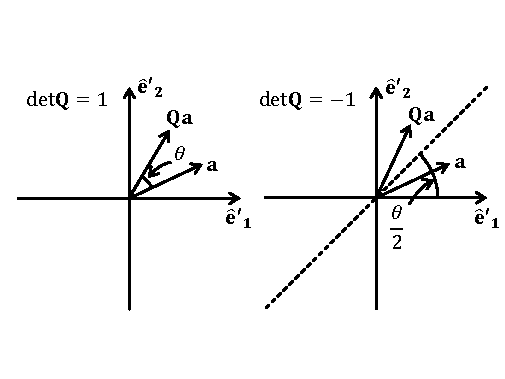
\includegraphics[width=0.5\textwidth]{images/II.3.1.pdf}
    \caption{正交算符在2维欧几里得空间中的几何意义。}
    \label{fig:II.3.1}
\end{figure}

接下来我们考虑$\mathrm{det}\mathbf{Q}=-1$时的情况。首先,$\mathbf{Q}$的两个特征值是1和$-1$。这相当于说$\mathrm{det}\left(\mathbf{Q}\pm\mathbf{I}\right)=0$。诚然,由算符的伴随的计算性质(定理\ref{thm:II.2.30}),$\left(\mathbf{Q}\pm\mathbf{I}\right)^*=\mathbf{Q}^*\pm\mathbf{I}$。由行列式的性质,$\mathrm{det}\left(\mathbf{Q}\pm\mathbf{I}\right)^*=\mathrm{det}\left(\mathbf{Q}\pm\mathbf{I}\right)$。再由
\begin{align*}
    \mathrm{det}\left(\mathbf{Q}\pm\mathbf{I}\right) & =\mathrm{det}\left(\mathbf{Q}\pm\mathbf{Q}^*\mathbf{Q}\right)                          \\
                                                     & =\mathrm{det}\left(\mathbf{Q}\right)\mathrm{det}\left(\mathbf{I}\pm\mathbf{Q}^*\right) \\
                                                     & =\left(-1\right)\left(-1\right)^2\mathrm{det}\left(\mathbf{Q}^*\pm\mathbf{I}\right)    \\
                                                     & =-\mathrm{det}\left(\mathbf{Q}^*\pm\mathbf{I}\right)
\end{align*}
可得$\mathrm{det}\left(\mathbf{Q}\pm\mathbf{I}\right)=-\mathrm{det}\left(\mathbf{Q}\pm\mathbf{I}\right)\Leftrightarrow\mathrm{det}\left(\mathbf{Q}\pm\mathbf{I}\right)=0$。

我们可进一步得到结论:行列式为$-1$的正交算符是对称算符。诚然,当$\mathrm{det}\mathbf{Q}=-1$时,设$\mathbf{\hat{e}}_1,\mathbf{\hat{e}}_2$分别是对应其特征值1和$-1$的单位特征向量,则$\left(\mathbf{\hat{e}}_1|\mathbf{\hat{e}}_2\right)=\left(\mathbf{Q\hat{e}}_1|\mathbf{Q\hat{e}}_2\right)=-\left(\mathbf{\hat{e}}_1|\mathbf{\hat{e}}_2\right)\Leftrightarrow\left(\mathbf{\hat{e}}_1|\mathbf{\hat{e}}_2\right)=0$。再由定理\ref{thm:II.2.32}的推论可得$\mathbf{Q}$是对称算符。

下面我们开始考察行列式为$-1$的对称算符的几何性质。沿用上一段的设定,在规范正交基$B=\left\{\mathbf{\hat{e}}_1,\mathbf{\hat{e}}_2\right\}$下,$\mathbf{Q}$的坐标矩阵将是以下对角矩阵
\[\left(\mathbf{Q}\right)_B=\left(\begin{array}{cc}1&0\\0&-1\end{array}\right)\]
但$B$是由$\mathbf{Q}$的性质规定的,一般不会恰巧就是我们讨论几何问题时选用的坐标系的基。设我们选用的是另一个有序规范正交基$B^\prime=\left\{\mathbf{\hat{e}}^\prime_1,\mathbf{\hat{e}}^\prime_2\right\}$,$P$是由$\mathbf{B}$到$\mathbf{B}^\prime$的过渡矩阵,则$P$也是一个正交矩阵。按照之前的结论,矩阵$P$可以某角度$\phi$表示成
\[P=\left(\begin{array}{cc}\cos\phi&\sin\phi\\\mp\sin\phi&\pm\cos\phi\end{array}\right)\]
事实上$\phi$是$\mathbf{\hat{e}}^\prime_1$与$\mathbf{\hat{e}}_1$的夹角。诚然,
\begin{align*}
    \left(\mathbf{\hat{e}}^\prime_1|\mathbf{\hat{e}}_1\right) & =\left(\sum_{k=1}^2P_{k1}\mathbf{\hat{e}}_k|\mathbf{\hat{e}}_1\right) \\
                                                              & =\sum_{k=1}^2P_{1k}\left(\mathbf{\hat{e}}_k|\mathbf{\hat{e}}_1\right) \\
                                                              & =P_{1k}\delta_{k1}=P_{11}=\cos\phi
\end{align*}

由之前的结论,$\mathbf{Q}$在$B^\prime$下的坐标可用某角$\theta$表示,同时又是通过矩阵$P$从其在$B$下的坐标变换而来的,故有以下关系
\begin{align*}
    \left(\mathbf{Q}\right)_{B^\prime} & =\left(\begin{array}{cc}\cos\theta&\sin\theta\\\sin\theta&-\cos\theta\end{array}\right) \\
                                       & =P^{\intercal}\left(\mathbf{Q}\right)_BP                                                \\
    \Leftrightarrow                    & \theta=2\phi
\end{align*}

设$\mathbf{a}=\alpha_1\mathbf{\hat{e}}^\prime_1+\alpha_2\mathbf{\hat{e}}^\prime_2$是二维欧几里得平面的任一平移向量。则$\mathbf{Qa}$在$B^\prime$下的坐标可由以下矩阵运算得到
\[\left(\mathbf{Q}\right)_{B^\prime}\left(\alpha_1,\alpha_2\right)^\intercal=\left(\begin{array}{c}\alpha_1\cos\theta+\alpha_2\sin\theta\\-\alpha_2\cos\theta+\alpha_1\sin\theta\end{array}\right)\]
记$\delta$为向量$\mathbf{a}$与$\mathbf{\hat{e}}^\prime_1$的夹角,则上式说明$\mathbf{Qa}$与$\mathbf{\hat{e}}^\prime_1$的夹角是$2\phi-\delta$。也就是说,在2维欧几里得平面上,任一向量被行列式为$-1$的正交算符$\mathbf{Q}$作用后的结果,是原向量关于角度为$\theta/2$的轴的镜象翻转。其中“角度”是指与所选定规范正交基的第1个单位基向量的夹角(图\ref{fig:II.3.1})。$\theta$是$\mathbf{Q}$在所选定的规范正交基下的坐标矩阵取前文所述的表达式时的角;它是$\mathbf{Q}$本身的特性。也就是说,当$\mathrm{det}\mathbf{Q}=-1$时,$\mathbf{Q}$在2维欧几里得空间中确定了一条镜象对称轴。特别地,当$\theta=0$时,意味着我们选取的直角坐标系第一条轴恰好是$\mathbf{Q}$确定的镜象对称轴。

\subsubsection{3维欧几里得平面上的几何意义}
设$\mathbf{Q}$是3维实内积空间$\mathcal{V}$中的正交算符,由其行列式的基本性质$\mathrm{det}\mathbf{Q}=\pm 1$,可知其3个特征值$\lambda_i=\pm 1,i=1,2,3$。设$\left\{\mathbf{\hat{e}}_1,\mathbf{\hat{e}}_2,\mathbf{\hat{e}}_3\right\}$是$\mathcal{V}$的一组规范正交基,且$\mathbf{\hat{e}}_1$是$\mathbf{Q}$的一个特征向量,即$\mathbf{Q\hat{e}}_1=\pm 1$。我们考察$\mathbf{Q}$在这组规范正交基下的坐标$Q_{ij}=\left(\mathbf{Q\hat{e}}_i|\mathbf{\hat{e}}_j\right)$,有如下结论
\begin{align*}
    \left(\mathbf{Q\hat{e}}_1|\mathbf{\hat{e}}_1\right)                                                                                                                      & =\pm 1                                                  \\
    \left(\mathbf{Q\hat{e}}_1|\mathbf{\hat{e}}_2\right)                                                                                                                      & =\left(\mathbf{Q\hat{e}}_1|\mathbf{\hat{e}}_3\right)=0, \\
    \left(\mathbf{Q\hat{e}}_2|\mathbf{\hat{e}}_1\right)=\left(\mathbf{\hat{e}}_2|\mathbf{Q}^*\mathbf{\hat{e}}_1\right)=\pm\left(\mathbf{\hat{e}}_2|\mathbf{\hat{e}}_1\right) & =0,
\end{align*}
其中用到了事实$\mathbf{Q}^*\mathbf{\hat{e}}_1=\pm\mathbf{\hat{e}}_1$,因为
\[\mathbf{\hat{e}}_1=\mathbf{Q}^*\mathbf{Q}\mathbf{\hat{e}}_1=\mathbf{Q}^*\left(\pm\mathbf{\hat{e}}_1\right)=\pm\mathbf{Q}^*\mathbf{\hat{e}}_1\]
同理有
\[\left(\mathbf{Q\hat{e}}_3|\mathbf{\hat{e}}_1\right)=0\]
换言之,我们得到了
\[Q_{11}=\pm 1,\quad Q_{12}=Q_{13}=Q_{21}=Q_{31}=0\]
另外注意到,$\left(\mathbf{Q\hat{e}}_i|\mathbf{\hat{e}}_j\right)$同时也是向量$\mathbf{Q\hat{c}}_i$的第$j$个坐标,故可知
\[\mathbf{Q\hat{e}}_2=Q_{22}\mathbf{\hat{e}}_2+Q_{23}\mathbf{\hat{e}}_3,\quad\mathbf{Q\hat{e}}_3=Q_{32}\mathbf{\hat{e}}_2+Q_{33}\mathbf{\hat{e}}_3\]
故由$\left\|\mathbf{Q\hat{e}}_2\right\|=\left\|\mathbf{\hat{e}}_2\right\|=\left\|\mathbf{Q\hat{e}}_3\right\|=\left\|\mathbf{\hat{e}}_3\right\|=1$有
\[Q_{22}^2+Q_{23}^2=Q_{32}^2+Q_{33}^2=1\]
由$\left(\mathbf{\hat{e}}_2|\mathbf{\hat{e}}_3\right)=0$有
\[Q_{22}Q_{32}+Q_{23}Q_{33}=0\]
由$\mathrm{det}\mathbf{Q}=\pm 1$有
\[-Q_{23}Q_{32}+Q_{22}Q_{33}=\pm 1\]
类似2维的情况,上述结论使我们可以把$\mathbf{Q}$在$\mathcal{V}$的任何一个以$\mathbf{Q}$的一个特征值为第一个单位基向量的有序基$B=\left\{\mathbf{\hat{e}}_1,\mathbf{\hat{e}}_2,\mathbf{\hat{e}}_3\right\}$下的坐标矩阵用某角$\theta$表达成
\[\left(\mathbf{Q}\right)_B=\left(\begin{array}{ccc}\pm 1&0&0\\0&\cos\theta&\sin\theta\\0&\mp\sin\theta&\pm\cos\theta\end{array}\right)\]
其中“$\pm$”表示当$\mathrm{det}\mathbf{Q}=1$时取正号,当$\mathrm{det}\mathbf{Q}=-1$时取负号。

以下我们考察,对任意向量$\mathbf{a}\in\mathcal{V}$,$\mathbf{Qa}$相比于$\mathbf{a}$在以$\mathcal{V}$为平移空间的欧几里得空间中的效果。

当$\mathrm{det}\mathbf{Q}=1$时,易验$\left(\mathbf{Qa}|\mathbf{\hat{e}}_1\right)=\left(\mathbf{a}|\mathbf{\hat{e}}_1\right)$,也就是说,$\mathbf{Q}$的作用不改变向量与$\mathbf{\hat{e}}_1$的夹角;$\mathbf{Qa}$与$\mathbf{a}$相比仅绕$\mathbf{\hat{e}}_1$旋转了一定的角度。具体地,设$\mathbf{a}=\sum_{i=1}^3\alpha_i\mathbf{\hat{e}}_i$,则
\[\mathbf{Qa}=\alpha_1\mathbf{\hat{e}}_1+\left(\alpha_2\cos\theta+\alpha_3\sin\theta\right)\mathbf{\hat{e}}_2+\left(-\alpha_2\sin\theta+\alpha_3\cos\theta\right)\mathbf{\hat{e}}_3\]
比较正交算符在2维欧几里得平面的分析结果,上式的后两项表示向量$\alpha_2\mathbf{\hat{e}}_2+\alpha_3\mathbf{\hat{e}}_3$在$\left(\mathbf{\hat{e}}_2,\mathbf{\hat{e}}_3\right)$所确定的平面上绕原点旋转了角$\theta$。联系格拉姆--施密特正交化过程可知,$\alpha_2\mathbf{\hat{e}}_2+\alpha_3\mathbf{\hat{e}}_3$就是向量$\mathbf{a}$在$\left(\mathbf{\hat{e}}_2,\mathbf{\hat{e}}_3\right)$所确定的平面上的投影向量。因此,当$\mathrm{det}\mathbf{Q}=1$时,$\mathbf{Qa}$在3维欧几里得空间确定了一个规范正交基$\left\{\mathbf{\hat{e}}_1,\mathbf{\hat{e}}_2,\mathbf{\hat{e}}_3\right\}$,其中$\mathbf{\hat{e}}_1$是一个旋转轴。对任意平移向量$\mathbf{a}$,$\mathbf{Qa}$在$\mathbf{\hat{e}}_2,\mathbf{\hat{e}}_3$所张的平面上的投影相比于$\mathbf{a}$在这一平面上的投影绕旋转轴旋转角$\theta$(图\ref{fig:II.3.2})。值得注意的是,$\left\{\mathbf{\hat{e}}_1,\mathbf{\hat{e}}_2,\mathbf{\hat{e}}_3\right\}$是由$\mathbf{Q}$的性质确定的。我们在讨论几何问题时未必恰好选择了这组特殊的规范正交基来建立直角坐标系。所以一般地,由$\mathbf{Q}$所定义的旋转轴在预先选定的直角坐标系中是“斜放”的。特别地,当$\theta=0$时,$\mathbf{Q}=\mathbf{I}$。

\begin{figure}[h]
    \centering
    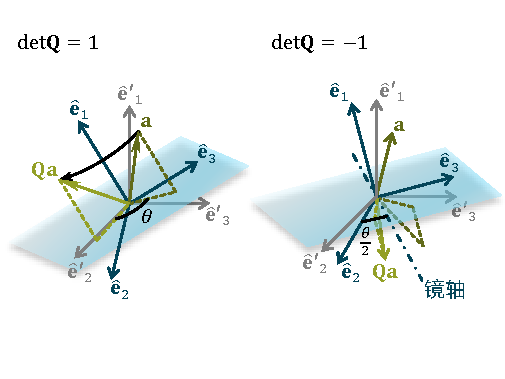
\includegraphics[width=0.5\textwidth]{images/II.3.2.pdf}
    \caption{正交算符在3维欧几里得空间中的几何意义。}
    \label{fig:II.3.2}
\end{figure}

当$\mathrm{det}\mathbf{Q}=-1$时,由类似的讨论可得
\[\mathbf{Qa}=-\alpha_1\mathbf{\hat{e}}_1+\left(\alpha_2\cos\theta+\alpha_3\sin\theta\right)\mathbf{\hat{e}}_2+\left(-\alpha_3\cos\theta+\alpha_2\sin\theta\right)\mathbf{\hat{e}}_3\]
首先,上式第一项说明,$\mathbf{Qa}$与$\mathbf{\hat{e}}_1$的夹角$\phi^\prime$跟$\mathbf{a}$与$\mathbf{\hat{e}}_1$的夹角$\phi$保持$\phi^\prime=\pi-\phi$的关系,也就是说$\mathbf{Qa}$把$\mathbf{a}$关于由$\left(\mathbf{\hat{e}}_2,\mathbf{\hat{e}}_3\right)$确定的平面进行了镜象翻转。然后,比较上式后两项与2维内积空间上的正交算符的分析结果可知,它们是$\mathbf{a}$在由$\left(\mathbf{\hat{e}}_2,\mathbf{\hat{e}}_3\right)$所确定的平面上,以与$\mathbf{\hat{e}}_2$夹角为$\theta/2$的直线为对称轴进行平面内的镜向翻转的结果(图\ref{fig:II.3.2})。总之,当$\mathrm{det}\mathbf{Q}=-1$时,$\mathbf{Q}$的几何效果就是上述两个操作的组合。$\mathbf{Q}$在3维欧几里得空间确定了一个镜面翻转的平面以及在该面内镜象翻转的一条对称轴。在已选定的直角坐标系中,这个平面和这条对称轴一般是“斜放”的。

\subsection{对称算符与向量的拉伸}\label{sec:II.3.3.2}
由定理\ref{thm:II.2.32},复数域上的厄米算符特征值全为实数。也就是说,厄米算符的特征多项式全为实根。因此,定理\ref{thm:II.2.32}中关于复数域上厄米算符的性质,也适用于在实数域上的对称算符,包括:特征值全都是实数\cite[\S 5.3 定理3.4]{周胜林2012线性代数};对应于不同特征值的特征向量必正交\cite[\S 5.3 定理3.5]{周胜林2012线性代数};必可对角化\cite[\S 5.3 定理3.6]{周胜林2012线性代数};存在一组规范正交基是其特征向量。

一个对称算符的3个特征向量两两正交。设对称算符$\mathbf{U}$的3个特征值为$\lambda_1,\lambda_2,\lambda_3$,$\mathbf{U}$的3个特征向量为$\mathbf{\hat{c}}_1,\mathbf{\hat{c}}_2,\mathbf{\hat{c}}_3$,在规范正交基$C=\left\{\mathbf{\hat{c}}_i\right\}$下,$\left(\mathbf{U}\right)_C$是一个对称矩阵
\[
    \left(\mathbf{U}\right)_C=\left(\begin{array}{ccc}\lambda_1&0&0\\0&\lambda_2&0\\0&0&\lambda_3\end{array}\right)
\]
在实际问题中我们未必方便选择$\mathbf{U}$的特征向量作为基。在其他规范正交基$B=\left\{\mathbf{\hat{e}}_i\right\}$下,$\left(\mathbf{U}\right)_B$是一个对称矩阵。

给定任一向量$\mathbf{a}=\sum_{i=1}^3\alpha_i\mathbf{\hat{c}}_i$,则有$\mathbf{Ua}=\sum_{i=1}^3\lambda_i\alpha_i\mathbf{\hat{c}}_i$。也就是说,与$\mathbf{a}$相比,$\mathbf{Ua}$是分别在$\mathbf{\hat{c}}_i$方向进行了比例为$\lambda_i$的拉伸或压缩,其中$i=1,2,3$。因此,任一对称算符$\mathbf{U}$均在3维空间中确定了1套(3个)两两正交的拉伸方向,以及在相应方向的拉伸比。我们把对称算符$\mathbf{U}$的单位特征向量$\left\{\mathbf{c}_i\right\}$在$\mathcal{E}$中所表示的方向称为该对称算符$\mathbf{U}$的\emph{主方向(principal direction)}。一组向量\footnote{在$\mathcal{E}$中,任何几何形状都是点的集合,而点又与位置向量一一对应,故任何几何形状都是一个向量组。}在对称算符的作用下的几何效果是在主方向上的拉伸。具体地,在$\mathbf{c}_i$方向的拉伸比就是$\lambda_i$。在预先选定的直角坐标系中,对称算符的主方向可能是“斜放”的。

特别地,当$\lambda_i=\pm 1,i=1,2,3$时,对称算符不改变形状的尺寸,但仍可能使形状发生翻转;因为此时对称算符要么是恒等算符,要么是行列式为$-1$的正交算符。

\subsection{斜称算符与向量的“叉乘”}\label{sec:II.3.3.3}
我们先比定理\ref{thm:II.2.32}更详细地考察斜称算符的性质。设$\mathcal{W}$是数域$\mathbb{F}$上的$n$维内积空间,$\mathbf{W}$是$\mathcal{W}$上的一个斜称算符,$\left\{\lambda_i\right\}$是$\mathbf{W}$的特征值。由定理\ref{thm:II.2.32},$\left\{\lambda_i\right\}$是纯虚数或零。在$\mathbb{R}^n$上,当$n$是奇数时,
\begin{align*}
                    & \mathrm{det}\mathbf{W}^\intercal=\mathrm{det}\mathbf{W}=\mathrm{det}\left(-\mathbf{W}\right)=\left(-1\right)^n\mathrm{det}\mathbf{W}=-\mathrm{det}\mathbf{W} \\
    \Leftrightarrow & \mathrm{det}\mathbf{W}=\prod_{i=1}^n\lambda_i=0
\end{align*}
故\emph{当$n$为奇数时,斜称算符必有一特征值为零}。而且,上列结果也说明,当$n$为奇数时,斜称算符不可逆(不满秩)。

现考虑3维的情况,改设$\mathbf{W}$是$\mathcal{V}$上的一个斜称算符,则对任意$\mathbf{a}\in\mathcal{V}$,
\[\left(\mathbf{Wa}|\mathbf{a}\right)=-\left(\mathbf{a}|\mathbf{a}\right)=\left(\mathbf{a}|\mathbf{Wa}\right)=-\left(\mathbf{a}|\mathbf{a}\right)\Leftrightarrow\left(\mathbf{Wa}|\mathbf{a}\right)=0\]
故被$\mathbf{W}$作用过的向量,都被投影到了与原向量垂直的平面上。至于投影了之后,有没有伸缩或旋转,要看$\mathbf{W}$的具体取值。这十分类似于以往所学过的一个向量被另一个向量“叉乘”的效果\footnote{3维实内积空间上的“叉乘”在以前的线性代数课本中又称作“向量的外积”\cite[\S3.2]{周胜林2012线性代数}。请复习其计算方法。}。事实上,我们可以从斜称算符定义“叉乘”\footnote{在本讲义中,将保持使用“叉乘”这种不正式的表述。因为正式起来,3维实内积空间上的“叉乘”是抽象代数中的不同东西在3维实内积空间上的巧合。在连续介质力学的数学语言中出现的“叉乘”,有时真的就是本节所述的几何意义,有时则是外代数/外积/楔积(如向量场的旋度)。本讲义暂时不介绍基于外代数和微分型知识,故“叉乘”运算就都由本节引入了。}。我们可通过如下定理联系二者:

\begin{theorem}\label{thm:II.3.1}
    设$\mathcal{V}$是实数域$\mathbb{R}$上的3维内积空间,$\mathbf{W}$是$\mathcal{V}$上的一个斜称算符,$\mathbf{\hat{e}}_1$是$\mathbf{W}$的关于特征值$\lambda=0$的一个特征单位向量。$\left\{\mathbf{\hat{e}}_i\right\}$是由$\mathbf{\hat{e}}_1$生成的规范正交基。对任意$\mathbf{a}\in\mathcal{V}$,可定义“叉乘”运算
    \[\mathbf{Wa}=\omega\mathbf{\hat{e}}_1\times\mathbf{a}\]
    其中$\omega=\left(\mathbf{W\hat{e}}_2|\mathbf{\hat{e}}_3\right)$。
\end{theorem}
\begin{proof}
    若记向量$\mathbf{W\hat{e}}_2=\sum_{i=1}^3\beta_i\mathbf{\hat{e}}_i$,即$\beta_i=\left(\mathbf{W\hat{e}}_2|\mathbf{\hat{e}}_i\right),\quad i=1,2,3$,则有
    \begin{align*}
        \beta_1 & =\left(\mathbf{W\hat{e}}_2|\mathbf{\hat{e}}_1\right)=-\left(\mathbf{\hat{e}}_2|\mathbf{W\hat{e}}_1\right)=\left(\mathbf{\hat{e}}_2|\mathbf{0}\right)=0     \\
        \beta_2 & =\left(\mathbf{W\hat{e}}_2|\mathbf{\hat{e}}_2\right)=-\left(\mathbf{e}_2|\mathbf{W\hat{e}}_2\right)\Leftrightarrow\beta_2=-\beta_2\Leftrightarrow\beta_2=0 \\
        \beta_3 & =\left(\mathbf{W\hat{e}}_2|\mathbf{\hat{e}}_3\right)=\omega
    \end{align*}
    因此向量$\mathbf{W\hat{e}}_2=\omega\mathbf{\hat{e}}_3$。类似的方法可得到$\mathbf{W\hat{e}}_3=-\omega\mathbf{\hat{e}}_2$。故对任意$\mathbf{a}\in\mathcal{V}$,
    \[
        \mathbf{Wa}=\alpha_1\mathbf{W\hat{e}}_1+\alpha_2\mathbf{W\hat{e}}_2+\alpha\mathbf{W\hat{e}}_3=\alpha_2\omega\mathbf{\hat{e}}_3-\alpha_3\omega\mathbf{\hat{e}}_2
    \]
    这恰为$\omega\mathbf{\hat{e}}_1\times\mathbf{a}$的结果
\end{proof}
要使用这个定理,就需要先已知$\mathbf{W}$,并找到$\mathbf{W}$在关于其零特征值的一个单位特征向量。如果我们先给定两个向量的“叉乘”$\mathbf{a}\times\mathbf{b}$,那么什么样的斜称算符$\mathbf{W}$满足$\mathbf{Wb}=\mathbf{a}\times\mathbf{b}$呢?答案作为\ref{thm:II.3.1}的推论如下。

\begin{corollary}
    设$\left\{\mathbf{\hat{e}}_i\right\}$是3维欧几里得空间$\mathcal{E}$的基本坐标系下已给定的一组有序规范正交基。给定向量$\mathbf{a}\in\mathcal{V},\mathbf{a}=\sum_{i=1}^3\alpha_i\mathbf{\hat{e}}_i$,则坐标矩阵为
    \[\left(\mathbf{W}\right)=\left(\begin{array}{ccc}0&\alpha_3&\alpha_2\\-\alpha_3&0&\alpha_1\\-\alpha_2&-\alpha_1&0\end{array}\right)\]
    的斜称算符$\mathbf{W}$满足$\mathbf{Wb}=\mathbf{a}\times\mathbf{b},\forall\mathbf{b}\in\mathcal{V}$。
\end{corollary}
该推论可利用坐标变换公式证明,可留作练习。另外,“叉乘”的性质$\mathbf{a}\times\mathbf{b}=-\mathbf{b}\times\mathbf{a}$也可通过在给定规范正交基下的坐标矩阵运算得到验证(仅限3维)。

一个斜称算符$\mathbf{W}$所对应的叉乘运算的第一个向量$\mathbf{a}$是由算符$\mathbf{W}$本身确定的,称为$\mathbf{W}$的\emph{轴向量(axial vetor)}。“叉乘”得到的向量,在坐标变换中的有特殊的性质。对任意$\mathbf{b}\in\mathcal{V}$,其在基本坐标系下的坐标是$\left(\beta_1,\beta_2,\beta_3\right)$。当我们反转各坐标轴的方向,即在$\left\{-\mathbf{\hat{e}}_i\right\}$下,$\mathbf{b}$的坐标将变号,变成$\left(-\beta_1,-\beta_2,-\beta_3\right)$,但是易验向量$\mathbf{a}\times\mathbf{b}$在坐标轴反转前后坐标不变号(请读者用坐标变换公式验证这两个结论)。同样的性质也导致“混合积”$\left(\mathbf{a}\times\mathbf{b}\right)\cdot\mathbf{c}$这一“标量”在坐标轴反转前后变号(而“真正的”标量的值不依赖坐标变换)。这是由于向量$\mathbf{a}\times\mathbf{b}$不是一个任意给定的孤立的向量;它是向量$\mathbf{b}$在以$\mathbf{a}$为轴向量的斜称算符$\mathbf{W}$的操作下的结果。由“叉乘”所得到的向量,其看上去特殊的坐标变换性质,实际上是这个投影操作带来的。有的资料称这种“叉乘得到的向量”为\emph{赝向量(pseudo-vector)}(但这不是该概念的正式定义)。
\end{document}